
\section{Model and Design}
\label{sec:model}


\begin{figure}[htb]
	\centering
	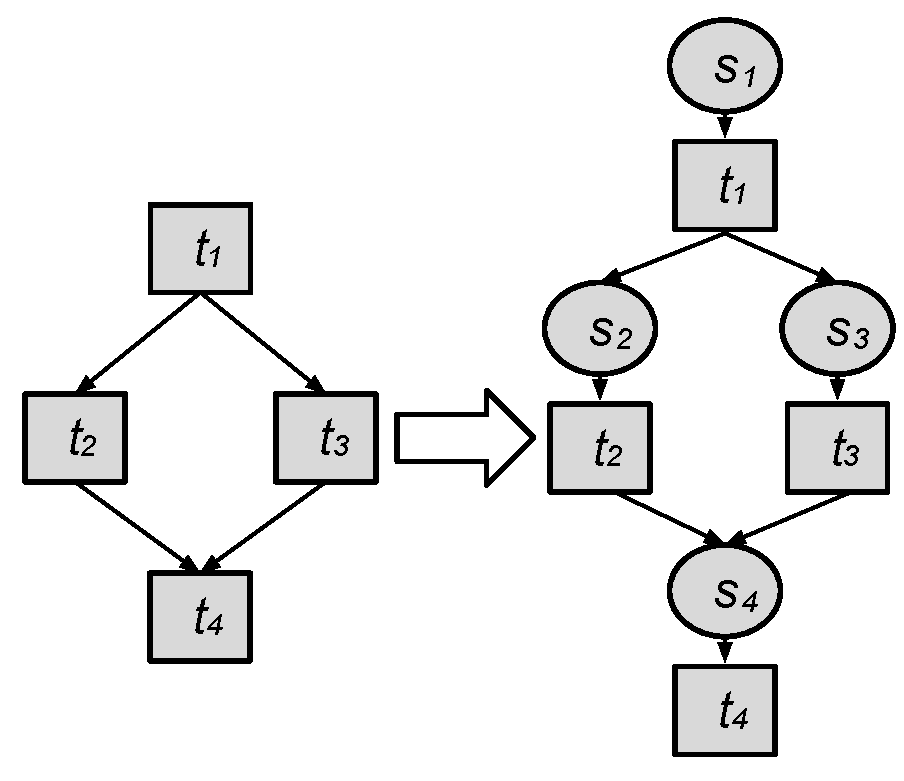
\includegraphics[width=0.7\linewidth]{figures/model/odag.pdf}
	\captionof{figure}{Extending DAG to o-DAG.}
	\label{fig:model_odag}
	\vspace{-10pt}
\end{figure}
A workflow is modeled as a Directed Acyclic Graph (DAG) as shown in Fig.~\ref{fig:model_odag} (Left). Each node in the DAG often represents a workflow job ($j$), and the edges represent dependencies between the jobs that constrain the order in which the jobs are executed. Dependencies typically represent data-flow dependencies in the application, where the output files produced by one job are used as inputs of another job. Each job is a single execution unit and it may contains one or multiple tasks, which is a program and a set of parameters that need to be executed. Fig.~\ref{fig:model_odag} (left) shows an illustration of a DAG composed by four jobs. This model fits several workflow management systems such as Pegasus~\cite{Deelman2005}, Askalon~\cite{Fahringer2005}, and Taverna~\cite{Oinn:2006:TLC:1148437.1148448}.

%Change it with job wrapper
Fig.~\ref{fig:model_system} shows a typical workflow execution environment. The submit host prepares a workflow for execution (clustering, mapping, etc.), and worker nodes, at an execution site, execute jobs individually. The main components are introduced below:

\begin{figure}[htb]
\centering
  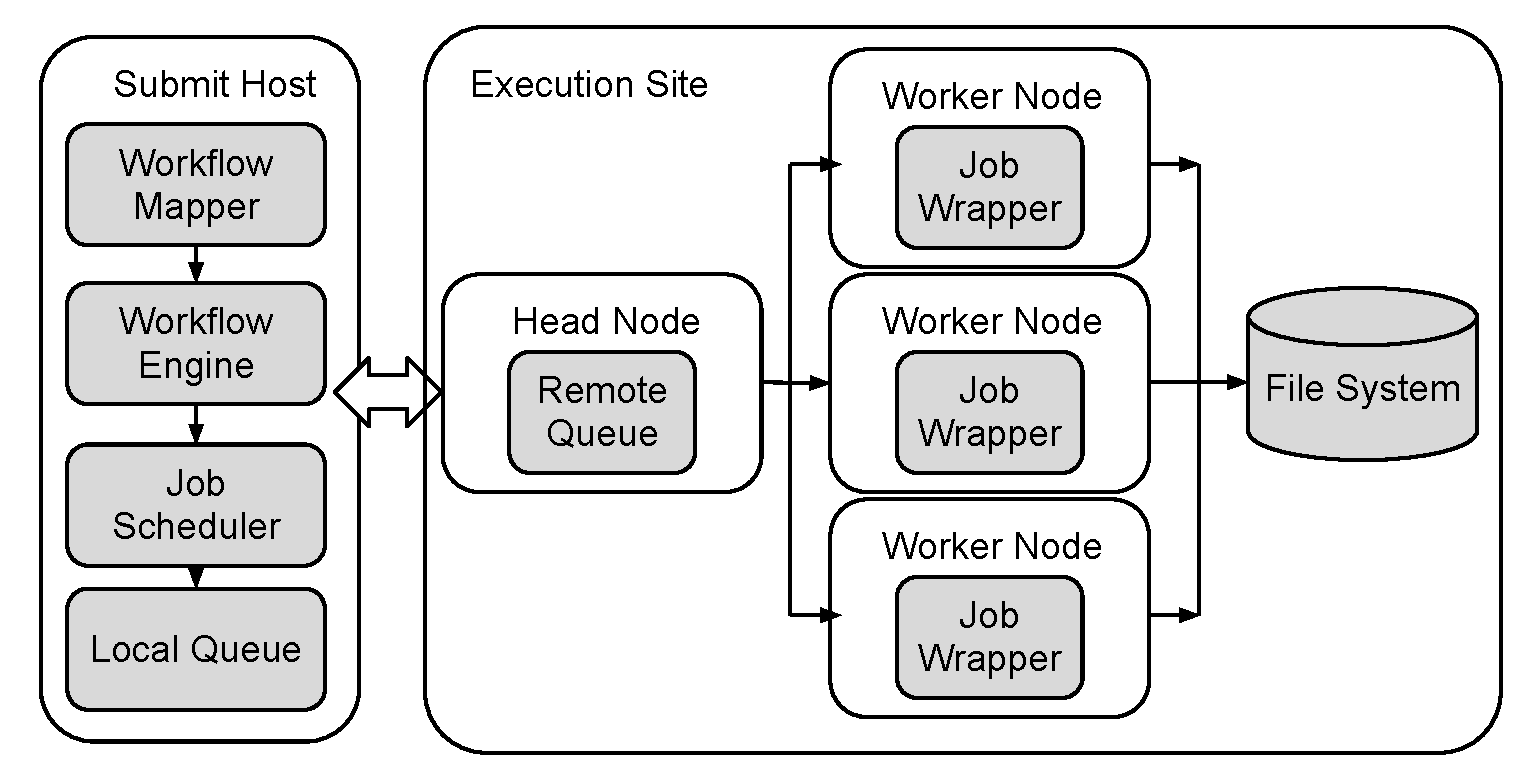
\includegraphics[width=0.95\linewidth]{figures/model/execution.pdf}
  \caption{A workflow system model.}
  \label{fig:model_system}
  \vspace{-10pt}
\end{figure}

\paragraph{Workflow Mapper} generates an executable workflow based on an abstract workflow provided by the user or workflow composition system. It also restructures the workflow to optimize performance and adds tasks for data management and provenance information generation. In this work, workflow mapper is particularly used to merge small tasks together into a job such that system overheads are reduced, which is called Task Clustering. A job is a single execution unit in the workflow execution systems and it may contain one or more tasks.

\paragraph{Workflow Engine} executes jobs defined by the workflow in order of their dependencies. Only jobs that have all their parent jobs completed are submitted to the Job Scheduler. Workflow Engine relies on the resources (compute, storage, and network) defined in the executable workflow to perform the necessary actions. The time period when a job is free (all of its parents have completed successfully) to when it is submitted to the job scheduler is denoted the workflow engine delay. The workflow engine delay is usually configured by users to assure that the entire workflow scheduling and execution system is not overloaded. 

\paragraph{Job Wrapper} extracts tasks from clustered jobs and executes them at the worker nodes. The clustering delay is the elapsed time on the extraction process.



\paragraph{Job Scheduler and Local Queue} manage individual workflow jobs and supervise their execution on local and remote resources. The time period when a job is submitted to the job scheduler to when the job starts its execution in a worker node is denoted the queue delay. It reflects both the efficiency of the job scheduler and the resource availability. 


\begin{figure}[h!]
	\centering
    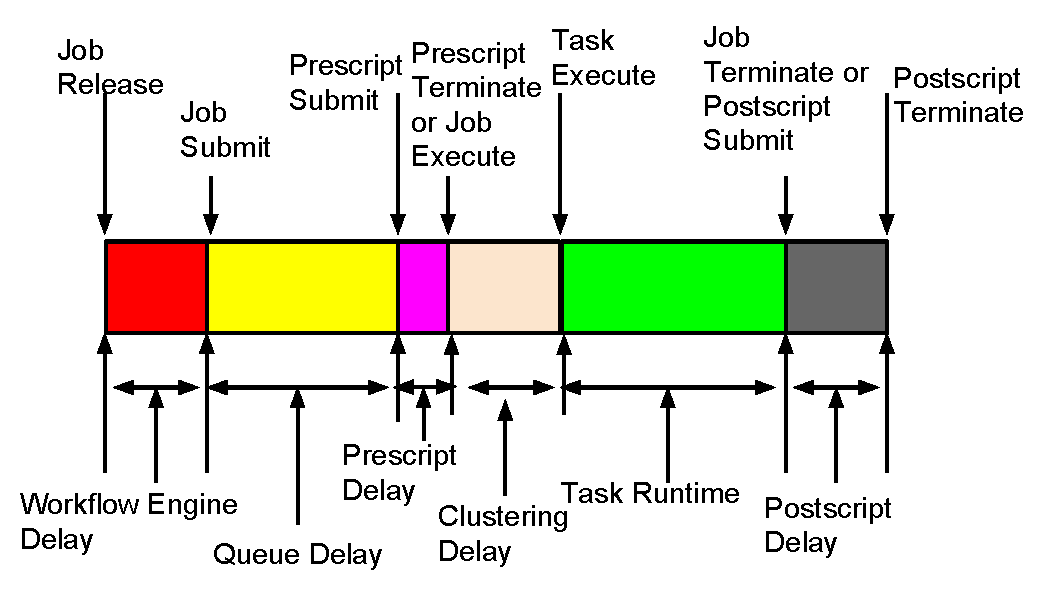
\includegraphics[width=0.5\textwidth]{figures/model/overhead.pdf}
    \caption{Workflow Events}
    \label{fig:model_overhead}
\end{figure}



The execution of a job is comprised of a series of events as shown in Fig.~\ref{fig:model_overhead} and they are defined as:

\begin{enumerate}
\item Job Release is defined as the time when the workflow engine identifies that a job is ready to be submitted (when its parents have successfully completed). 
\item Job Submit is defined as the time when the workflow engine submits a job to the local queue. 
\item Job Execute is defined as the time when the workflow engine sees a job is being executed. 
\item Task Execute is defined as the time when the job wrapper sees a task is being executed. 
\item Pre/Postscript Start is defined as the time when the workflow engine starts to execute a pre/postscript. 
\item Pre/Postscript Terminate is defined as the time when the pre/postscript returns a status code (success or failure). 
\end{enumerate}

Fig.~\ref{fig:model_overhead} shows a typical timeline of overheads and runtime in a compute job. We do not specify the data transfer delay in this timeline because data transfer is handled by data transfer jobs (stage-in and stage-out jobs). 

As shown in our prior work \cite{Chen2011}, we have classified workflow overheads into four categories as follows. 
\begin{enumerate}

\item{Workflow Engine Delay} measures the time between when the last parent job of a job completes and the time when the job gets submitted to the local queue. The completion time of the last parent job means this job is released to the ready queue and is waiting for resources to be assigned to it. The workflow engine delay reflects the efficiency of a workflow engine (i.e., DAGMan~\cite{DAGMan}). 

\item{Queue Delay} is defined as the time between the submission of a job by the workflow engine to the local queue and the time the local scheduler sees the job running. This overhead reflects the efficiency of the local workflow scheduler (e.g. Condor \cite{Frey2002}) to execute a job and the availability of resources for the execution of this job. 

\item{Pre/Postscript Delay } is the time taken to execute a lightweight script under some execution systems before/after the execution of a job. For example, prescripts prepare working environment before the execution of a job starts and postscripts examine the status code of a job after the computational part of this job is done.

\item{Clustering Delay} measures the difference between the sum of the actual task runtime and the job runtime seen by the job wrapper. The cause of Clustering Delay is usually because we use a job wrapper in worker nodes to execute a clustered job that requires some delay to extract the list of tasks. 

\end{enumerate}

The overhead aware DAG model (o-DAG) we use in this work is an extension of the traditional DAG model. System overheads play an important role in workflow execution and constitute a major part of the overall runtime when jobs are poorly mapped to resources. Fig.~\ref{fig:model_odag} shows how we augment a DAG to be an o-DAG with the capability to represent system overheads ($s$) such as workflow engine delay and queue delay.  In summary, an o-DAG representation allows the specification of high level system overhead details, which is more suitable for the study of overhead aware scheduling. 